\documentclass[11pt,landscape,a4paper]{article}
\usepackage[top=7mm,bottom=7mm,left=7mm,right=7mm]{geometry}
\usepackage[utf8]{inputenc}
\usepackage[ngerman]{babel}
\usepackage[T1]{fontenc}
\usepackage{amsmath}
\usepackage{amssymb}
\usepackage{bbm}
\usepackage[nosf]{kpfonts}
\usepackage[t1]{sourcesanspro}
\usepackage{multicol}
\usepackage{wrapfig}
\usepackage[framemethod=tikz]{mdframed}
\usepackage{microtype}
\usepackage{pdfpages}
\usepackage[shortlabels]{enumitem}

\newif\iflong
\longtrue % \longfalse for short version and \longtrue for long version
\newcommand{\inLongVersion}[1]{\iflong #1\fi}

\setlist{nosep}
\setlist[itemize]{leftmargin=*}
\setlist[enumerate]{leftmargin=*}

\newcommand{\R}{\mathbb{R}}
\newcommand{\E}{\mathbb{E}}
\renewcommand{\P}{\mathbb{P}}
\newcommand{\No}{\mathcal{N}}
\newcommand{\Mo}{\mathcal{M}}
\newcommand{\Do}{\mathcal{D}}
\DeclareMathOperator{\cov}{\operatorname{Cov}}
\DeclareMathOperator{\var}{\operatorname{Var}}
\DeclareMathOperator{\argmin}{\operatorname{argmin}}
\DeclareMathOperator{\argmax}{\operatorname{argmax}}
\DeclareMathOperator{\sgn}{\operatorname{sgn}}
\let\bar\overline

\begin{document}
\definecolor{blue}{cmyk}{0,0,0,1}
\definecolor{red}{rgb}{255,0,0}

\newcommand\Warning{%
   \makebox[1.4em][c]{%
      \makebox[0pt][c]{\raisebox{.1em}{\small!}}%
      \makebox[0pt][c]{\color{red}\Large$\bigtriangleup$}}
}%

\pgfdeclarelayer{background}
\pgfsetlayers{background,main}

\everymath\expandafter{\the\everymath \color{blue}}
\everydisplay\expandafter{\the\everydisplay \color{blue}}

\renewcommand{\baselinestretch}{.85}
\pagestyle{empty}

\global\mdfdefinestyle{header}{%
   linecolor=gray,linewidth=1pt,%
   leftmargin=0mm,rightmargin=0mm,skipbelow=0mm,skipabove=0mm,
}

\newcommand{\header}{
   \begin{mdframed}[style=header]
      \footnotesize
      \sffamily
      \centering
      ~Page~\thepage
   \end{mdframed}
}

\makeatletter % Author: https://tex.stackexchange.com/questions/218587/how-to-set-one-header-for-each-page-using-multicols
\renewcommand{\section}{\@startsection{section}{1}{0mm}%
   {.5ex}%
   {.2ex}%x
   {\color{blue}\sffamily\bfseries\large}}
\renewcommand{\subsection}{\@startsection{subsection}{2}{0mm}%
   {.2ex}%
   {.2ex}%x
   {\sffamily\bfseries}}
\renewcommand{\subsubsection}{\@startsection{subsubsection}{3}{0mm}%
   {.1ex}%
   {.1ex}%x
   {\sffamily\itshape}}
\makeatother


\setlength{\parindent}{5pt}
\setlength{\abovedisplayskip}{2pt}
\setlength{\belowdisplayskip}{2pt}
\setlength{\abovedisplayshortskip}{0pt}
\setlength{\belowdisplayshortskip}{0pt}

\small
\begin{multicols*}{4}
    \section{Adversarial Attacks}
\textbf{Targeted FGSM:} $x^\prime = x - \varepsilon \sgn(\nabla_x \mathcal{L}_t(x))$, where $t$ is the target label.

\textbf{Untargeted FGSM:} $x^\prime = x + \varepsilon \sgn(\nabla_x \mathcal{L}_y (x))$, where $y$ is the original label.

\textbf{Carlini-Wagner:}\\
Solve $\argmin_\eta ||\eta||_p+\lambda \mathcal{L}_t(x+\eta)$ s.t. $x+\eta\in [0,1]^n$. $\mathcal{L}$ satisfies $\mathcal{L}_t(x+\eta)\le 0 \Rightarrow f(x+\eta)=t$. Optimized with LBFGS-B. Replace $\|\cdot\|_{\infty}$ by $\sum_i \max(\eta_i-\tau,0)$ for faster convergence (updates multiple coordinates at once).

\textbf{PGD:} Iterate FGSM, each time with a small step. Typically used for adversarial training.

\textbf{Adv. Accuracy:} $\frac{\#\text{correct class and no adv example}}{\#\text{samples}}$

\textbf{Defense:} $\min_\theta \E_{x,y} [\max_{x^\prime\in S(x)} \mathcal{L}(x^\prime, y; \theta)]$.

\textbf{Norms}:
\begin{itemize}
    \item[] $\|x\|_\infty\leq\|x\|_1\leq d\|x\|_\infty$
    \item[] $\|x\|_\infty\leq\|x\|_2\leq\sqrt{d}\|x\|_\infty$
    \item[] $\|x\|_2\leq\|x\|_1\leq\sqrt{d}\|x\|_2$
    \item[] Hölder: $\|fg\|_1\leq\|f\|_p\|g\|_q$ \text{ if } $\frac{1}{p}+\frac{1}{q}=1$
\end{itemize}

    \section{Certification}
Goal: given a neural network $N$, a constraint over input $\phi$ and a property over outputs $\psi$, prove that $i \vDash \phi \Rightarrow N(i) \vDash \psi$ or return a violation. We want sound, complete and scalable algorithms, i.e., to either scale sound and complete methods or to make sound but incomplete methods more complete.
\begin{itemize}
    \item If the property does not hold, the program always states the property does not hold.
    \item If the property holds, the program always states the property holds.
\end{itemize}

\subsection*{Convex Relaxations}
Incomplete but sound
\begin{itemize}
    \item Box. Use hypercubes as approximation.
          % \item Zonotope. Represent every variable by $x_i = a^i_0+\sum_j a_j^i \epsilon_j = a_i^T e$, where $\epsilon_i\in [-1,1]$, $a_i\ge 0$. (1) The encoding for affine layer $y=Wx+b$ is $y=W A e+b$, which is exact. (2) To compute the encoding for ReLU layers, we first obtain box bounds by plugging in $\epsilon=-1$ and $\epsilon=1$. When it is strictly positive (negative), then use $y=x$ ($y=0$). For cross-boundary cases, use the line between $(l,0)$ and $(u,u)$ as the upper bound ($y=\lambda(x-l)$, $\lambda=\frac{u}{u-l}$) and its parallel as the lower bound ($y=\lambda x$). Then we compute the standard form of this zonotope by $y = \lambda(x-tl)$, $t\in [0,1]$, plug in $t=(\epsilon_{\text{new}}+1)/2$, $\epsilon_{\text{new}}\in [-1,1]$ and expand.
    \item DeepPoly. Bound every variable by $\sum_j w^l_jx_j + v^l \leq x_i \leq \sum_j w^u_j x_j +v_j$ and $l_i \le x_i \le u_i$. First do a forward propagation and then a backward propagation. (1) For affine layer $y=Wx+b$, use $Wx+b\le y\le Wx+b$. (2) For ReLU layers, if it is strictly positive (negative), use $x\le y\le x$ ($0\le y\le 0$). Otherwise, apply min-area heuristic to choose one from $0\le y\le \lambda(x-l)$ and $\lambda x\le y \le \lambda(x-l)$ (where $\lambda=\frac{u}{u-l}$), i.e., choose the first one if $u\leq -l$ o.w. the second one. When forward-propagating, we compute the interval bound by backsubstituting to the first layer.
\end{itemize}

Relaxations of methods not included in one another cannot be compared.

\subsection*{MILP}
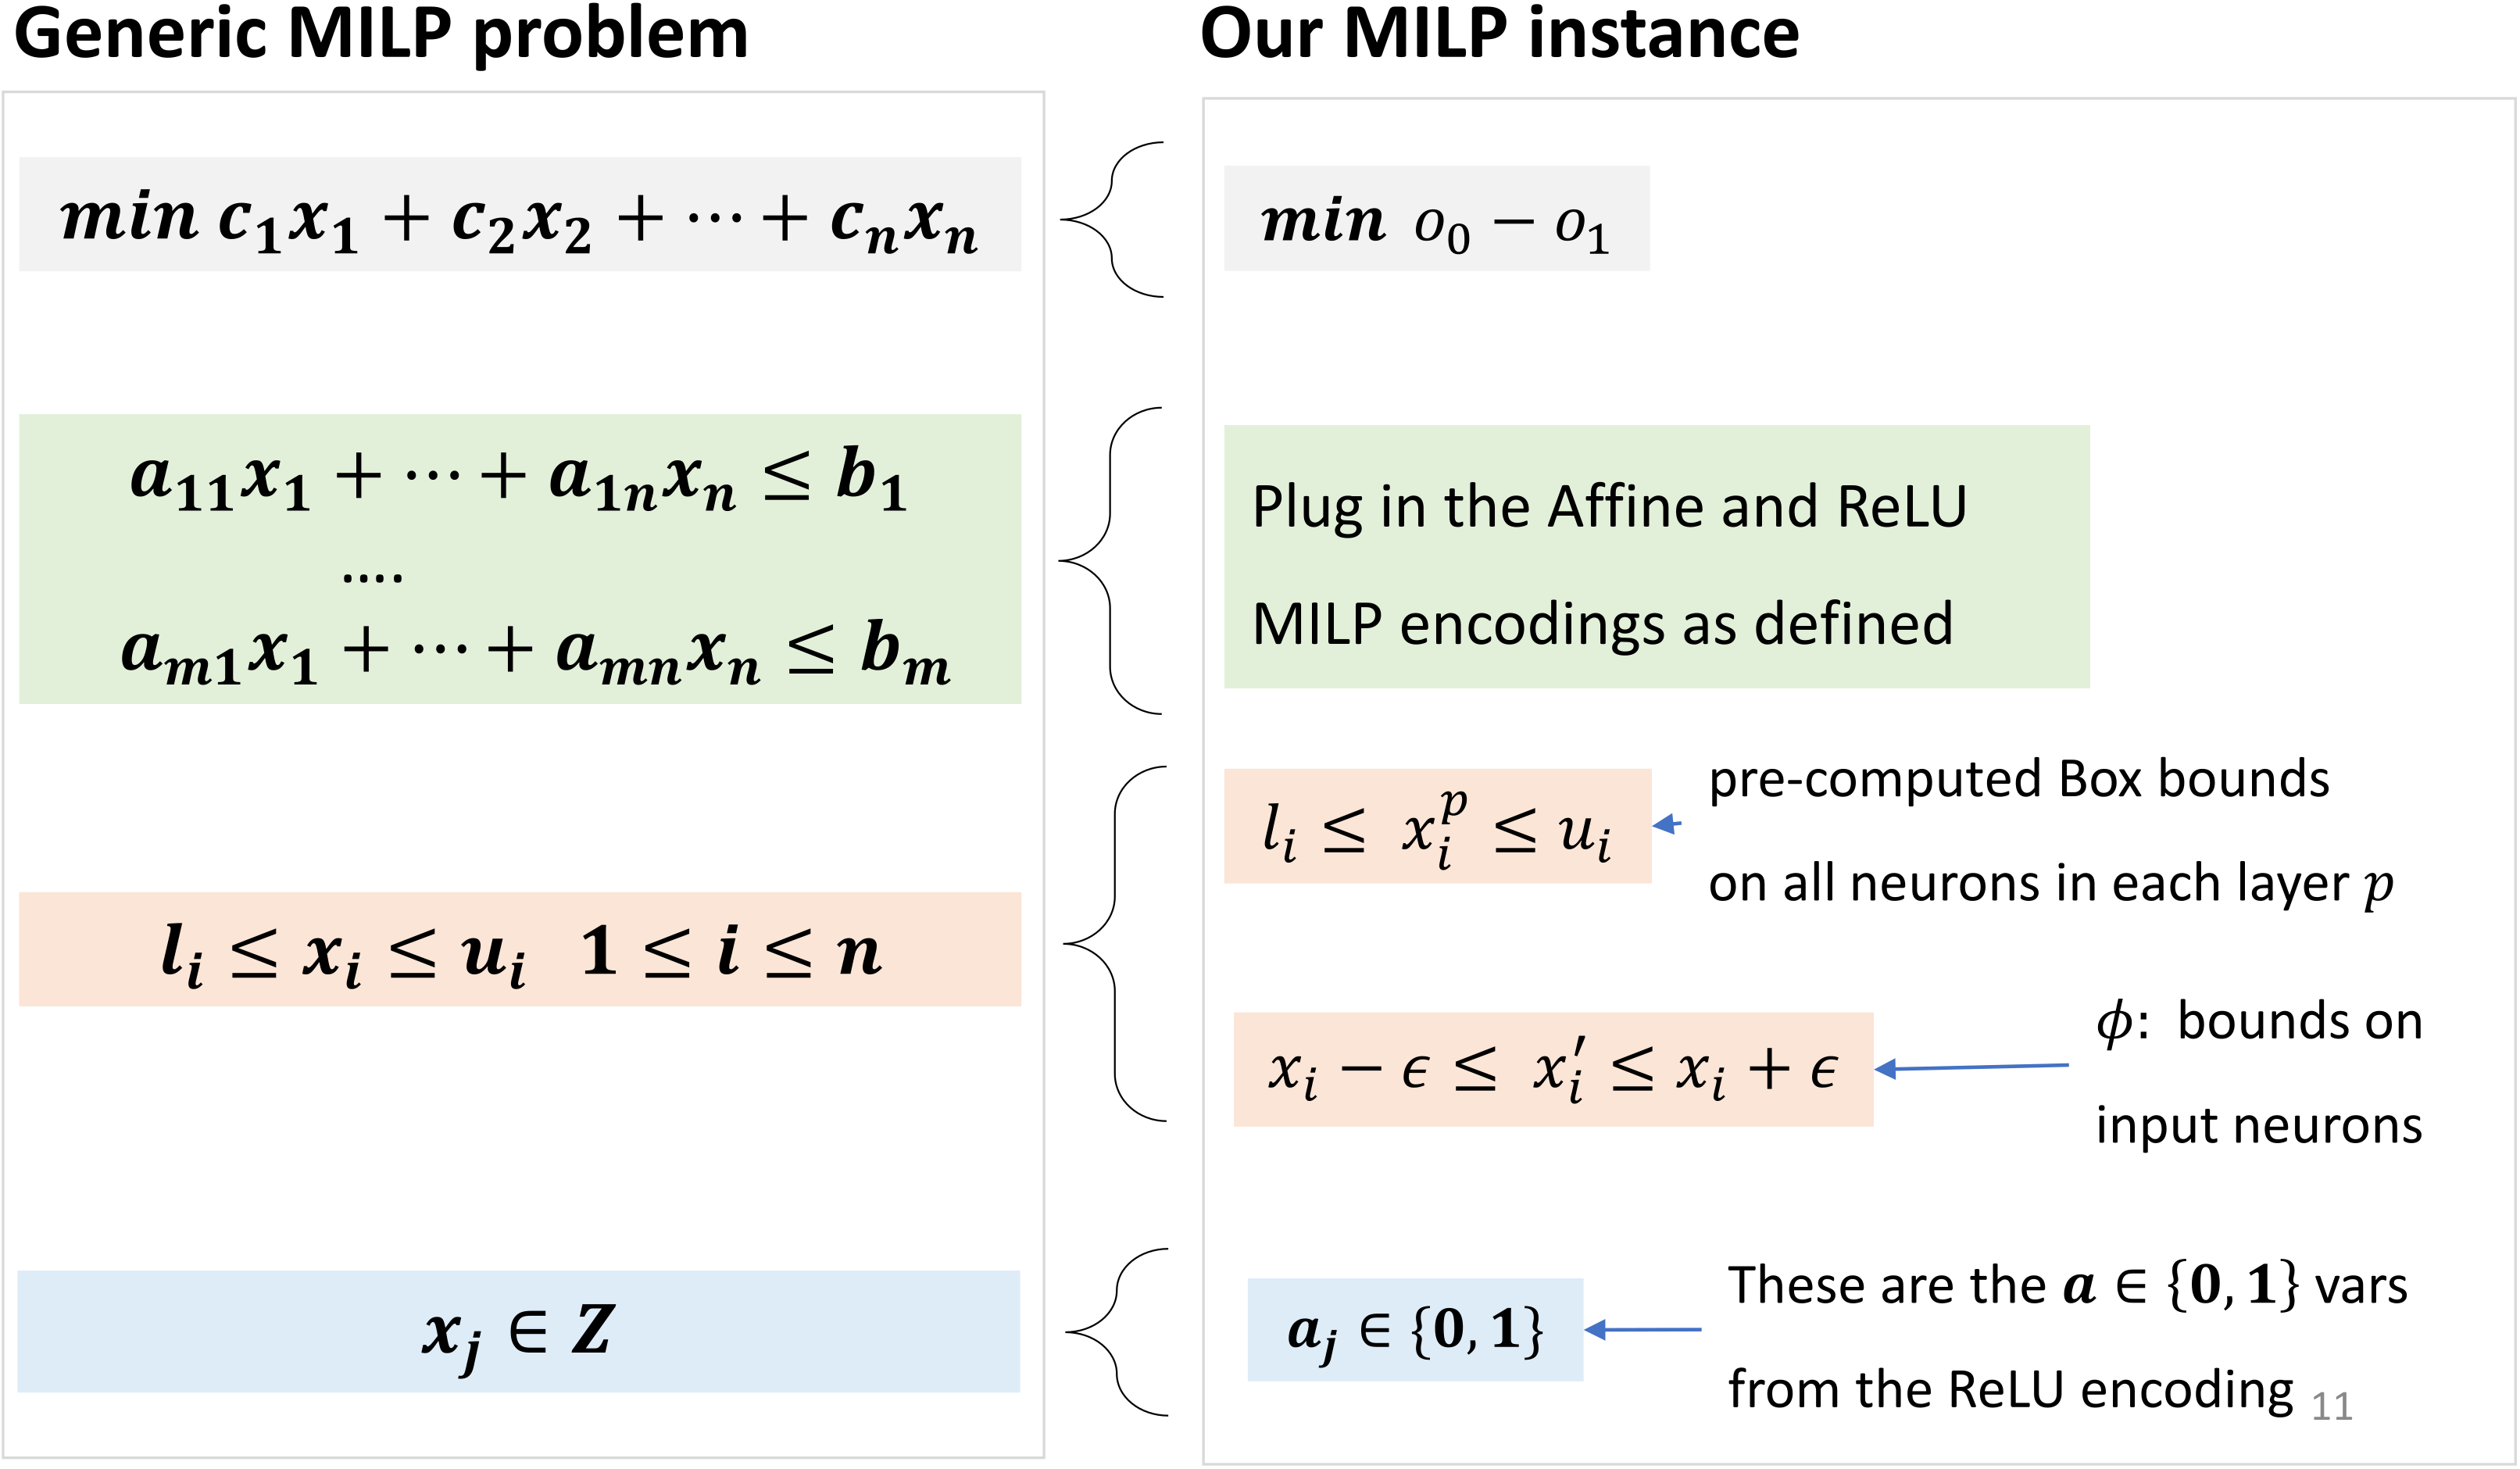
\includegraphics[width=1\linewidth]{img/milp.png}
Complete and sound for ReLU network, but is NP-complete.

The encoding for \textbf{affine} layer is: $Wx+b\le y\le Wx+b$. The encoding for \textbf{ReLU} is: $x\leq y\leq x-l(1-a)$,  $y\le ua$, $y\ge 0$ and $a\in\{0,1\}$. The variable $a$ serves as a ``state'' indicator to encode a piece-wise linear function. The bounds $l,u$ are pre-computed by Box. MILP benefits from Box bounds in that it could stop further exploration of infeasible combinations of integer variables, e.g., if the objective lower bound is positive when $a_1=0$, then there is no need to explore $a_2$ for $a_1=0$.

\subsection*{Branch and Bound}
Can split variables in cases (e.g. \nolinebreak{ReLU} output can be positive or negative) and certify both splits separately. Constraints can be enforced using KKT condition.
% \vspace*{-3mm}
\begin{center}
    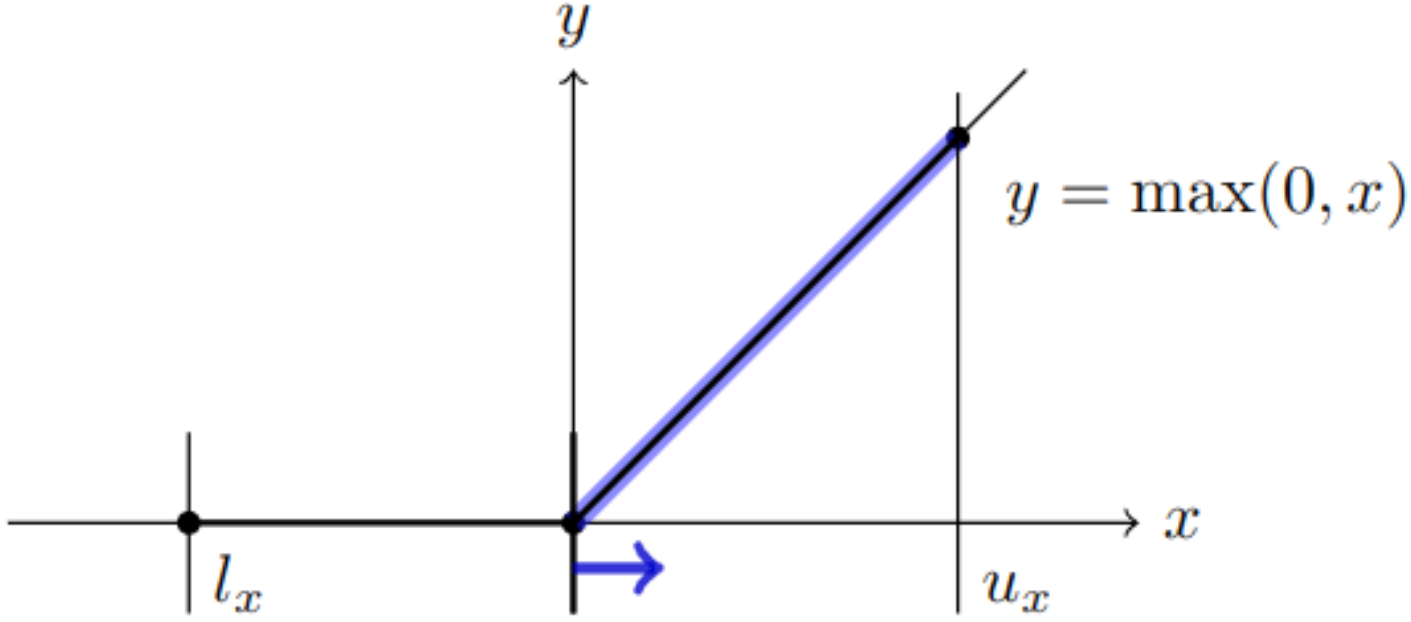
\includegraphics[width=.6\linewidth]{img/bnb.png}
\end{center}
% \vspace*{-2mm}
\begin{equation*}
    \begin{split}
        \max_{x\in\mathcal{X}} \  &a^\top x+c\leq \max_{x\in\mathcal{X}}\min_{\beta\geq0}a^\top x+c+\beta x_i \\[-2mm]
        \text{s.t.} \ \ \        &  x_i\geq0
    \end{split}
\end{equation*}
\Warning Adjust output bounds when splitting.

Initialize queue (without splits). While queue is not empty and not timed out:
1. Get subproblem from queue.
2. Compute bound of interest.
3. If not verified, pick neuron to split according to heuristic.
4. Add both new subproblems to queue.

    \section{Certified Training}
Goal: $\min_\theta\mathbb{E}_{(x,y) \sim D} \big[ \max\limits_{{x' \in B_\varepsilon(x)}} \mathcal{L}(\theta, {x'}, y) \big]$\\
\subsection*{DiffAI / IBP}
IBP (over)approximates inner max by propagating the box $B_\varepsilon(x)$ and computing the max loss over the output set. Can use any abstract transformer (Box, DeepPoly, etc.) to get bounds on logits.

\subsection*{SABR}
SABR uses the loss\\ $$\mathcal{L}_{\varepsilon,\tau}(x,y)=\max_{x'\in B_{\varepsilon-\tau}(x)} \max_{z\in B_\tau(x')}CE(f(z),y),$$
i.e. it uses a box $B_\tau(x')$ of size $\tau \leq\varepsilon$ around an adversarial sample $x'$. The outer max is (under)approximated by PGD search and the max inside is (over)approximated using IBP.

% \textbf{DiffAI}
% $$\min_\theta \E_{x,y} \max_{z\in \gamma(NN^{\#}(S(x)))} \mathcal{L}(z, y;\theta)$$
% where $S(x)$ is the allowed input set, $NN^{\#}$ is the abstraction of NN (e.g., DeepPoly abstraction).
% \begin{itemize}
%     \item Suppose we use $\mathcal{L}(z, y) = \max_{q\ne y}(z_q-z_y)$. Then for each iteration, we first compute the convex relaxation of the input, and then compute the interval bound for $z_q-z_y$. Then we use the upper bound as the loss and update according to the gradient (Note that it is still differentiable).
%     \item Suppose we use the cross entropy loss. Then we first compute the interval bound for $z_i$ and pick the upper bound for incorrect classes and lower bound for correct classes to form a new vector. Then we use this new vector to compute the cross entropy and update.
% \end{itemize}
% Practical tricks: (1) Annealing: start with a small $S(x)$ and then grow it. (2) Dynamically switch between standard loss and the certified loss.

% Convex Layerwise Adversarial Training (\textbf{COLT}) avoids increasing difficulty in the optimization due to better relaxations. The goal is to find a feasible point in the first-layer relaxation so that the loss is maximized and use this feasible point in the certified loss. When combined with Zonotope, it uses projection in the $\epsilon$ space since each $\epsilon \in [0,1]^n$ corresponds to a point in the zonotope. Although it is not the min-distance projection in the zonotope, it avoids the problem when the zonotope lies in a lower dimension where direct projection is not possible. It allows better results when a better relaxation is used.

% To find inner max, use abstract loss $\mathcal{L}(\vec{z}, y)$, where $y = $ target label, $\vec{z} = $ vector of logits:
% \begin{itemize}
%     \item $\mathcal{L}(z, y) = \max_{q \neq y} (z_q - z_y)$: Compute {$d_c = z_c - z_y \forall c \in \mathcal{C}$} where $\mathcal{C}$ set of classes and $z_c$ the abstract logit shape of class $i$. Then compute box bounds of $d_c$ and compute max upper bound: {$\max_{c \in \mathcal{C}}(\max(box(d_c)))$}
%     \item $\mathcal{L}(z,y) = CE(z,y)$: Compute box bounds $[l_c, u_c]$ of logit shapes $z_c$. $\forall c \in \mathcal{C}$ pick $u_c$ if $c \neq y$, pick $l_c$ if $c = y$. Then compute $CE(\operatorname{softmax}(v), y)$ where $v = [u_0, u_1,.., l_c,.., u_{|\mathcal{C}|}]$.
% \end{itemize}
% Cheap relaxations (e.g. Box) scale but introduce lots of infeasible points. Results in big drop in accuracy.
% Empirically, more precise relaxations (Zonotope) do not actually bring better results in provabililty. Hypothesis: more complex abstractions lead to more difficult optimization problems.
    \section{Randomized Smoothing}

Given a classifier $f$ and $\epsilon \sim \No(0,\sigma^2 I)$, define a smoothed classifier $g$ as
$$g(x)=\argmax_c \P\left[f(x+\epsilon)=c\right].$$\noindent
\textbf{THM:} Suppose $\exists {p_A}, {p_B} \in [0,1]$, s.t. $\P\left[f(x+\epsilon)=c_A\right] \ge {p_A} \ge {p_B} \ge \max_{c\ne c_A} \P\left[f(x+\epsilon)=c\right].$ Then $g(x+\delta)=c_A$ for all $\|\delta\|_2 <R$, where the radius $R=\frac{\sigma}{2} (\Phi^{-1}({p_A})-\phi^{-1}({p_B}))$ and $\Phi^{-1}$ is the Gaussian quantile function.

If we have ${p_A}>\frac{1}{2}$, then ${p_B}\leq1-{p_A}<p_A$ and thus $R>\sigma \Phi^{-1}({p_A})$. To compute probability, we use sampling. To avoid selection bias, we first sample to get the top label and then use an independent sampling to estimate the probability:

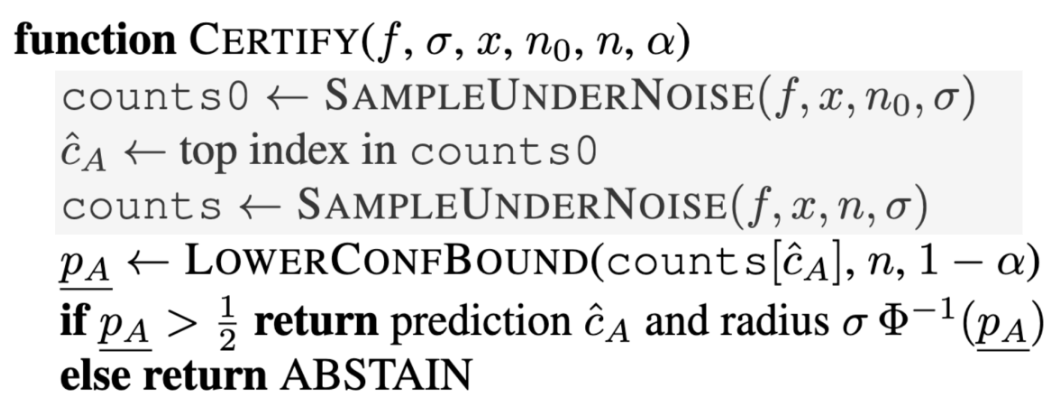
\includegraphics[width=\columnwidth]{img/rand_smooth.png}

By the above theorem, we have $g(x)=\hat{c}_A$ for all $\|\delta\|_2 <R$
with probability $1-\alpha$ if $\hat{c}_A, R$ is returned.

For inference, to compute $g(x)$, we use:

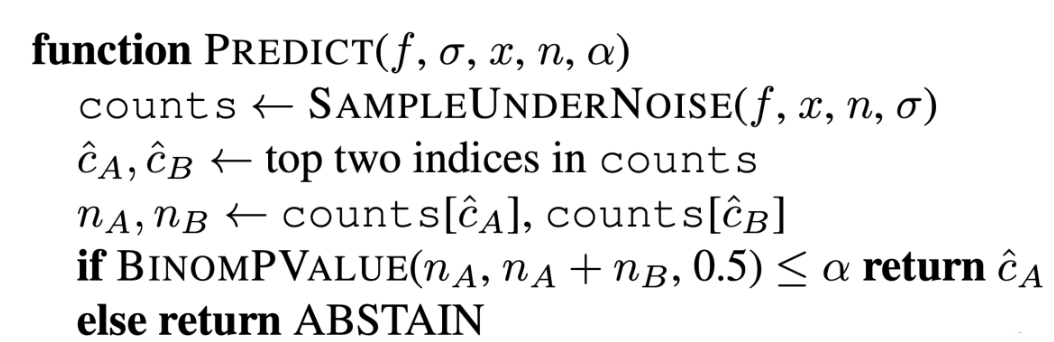
\includegraphics[width=\columnwidth]{img/rand-predict.png}

The probability of wrong prediction is $\P\left[\hat{c_A}\ne c_A, \text{no abstain}\right] = \P\left[\text{no abstain} \mid \hat{c_A}\ne c_A\right] \P\left[\hat{c_A}\ne c_A\right]\le \alpha$.

Pros: (1) it can scale to large networks and (2) is model-agnostic.

Cons: (1) it requires sampling at inference time and (2) many samples could be needed to increase the certified radius.

\textbf{Standard Gaussian CDF} \ \ $\Phi(a)=\P\left[X\le a\right]$
\begin{itemize}
    \item[] $1-\Phi(a)=\Phi(-a)$
    \item[] $\Phi^{-1}(1-p)=-\Phi^{-1}(p)$
\end{itemize}
    \section{Federated Learning}
% Types of Federated Learning:
% \begin{enumerate}
%     \item Cross-device. (1) Huge \#sources, (2) each with small amount of data, (3) dynamically drop in and out in the learning process, (4) contact rarely. Example: Google spell checker.
%     \item Cross-sillo. (1) Limited \#sources, (2) each with a lot of data, (3) participate constantly, (4) potentially heterogeneous. Example: Hospitals MRI segmentation.
% \end{enumerate}
Communication Round: (1) Server selects clients to participate. (2) Clients do local training update on private data and send information to the server. (3) Server aggregates updates into updated model.

\subsection*{FedSGD}
Clients compute gradient wrt. (minibatch of) local data on global weights. Server takes average for global update. Pros: convergence guarantee. Cons: requires lots of communication. Gradient inversion:
\begin{center}
    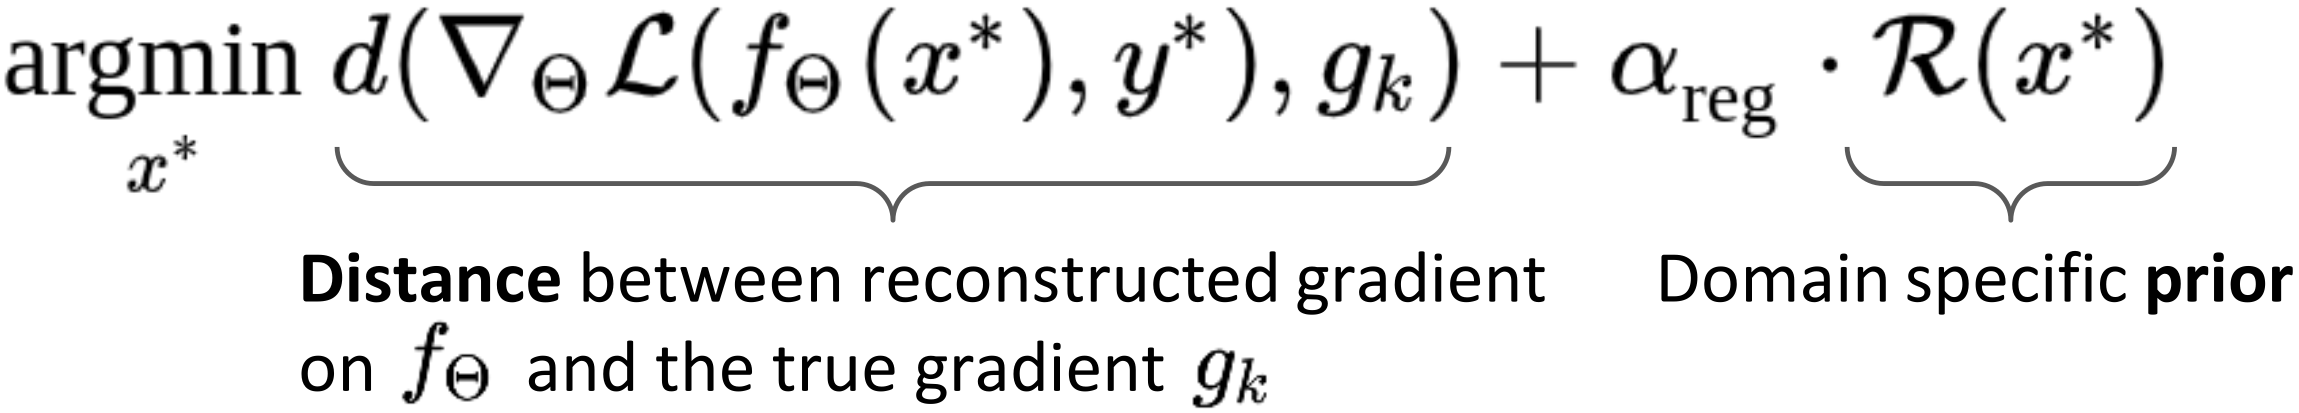
\includegraphics[width=0.7\linewidth]{img/gradient_inversion.png}
\end{center}
% \vspace*{-3mm}

\subsection*{FedAvg} Do several iterations of local SGD on the global weights and average the local weights as the global weight. Pros: Less communication. Cons: No convergence guarantee.

% \subsection*{Issues}
% \begin{itemize}
%     \item Honest-but-Curious Server: honestly follow the algorithm but want to expose private data of clients. Gradient inversion: match gradients of reconstructed and client data.
%     \item Client-side poisoning: send crafted updates to the server to force divergence or bad behavior on certain data.
%     \item Client fairness: model behaves well on average but poorly for certain clients due to heterogeneity. There is a trade-off between preventing client-side poisoning and client fairness because the server cannot tell whether a bad update is malicious or because of heterogeneity.
% \end{itemize}
    \section{Privacy}
\subsection*{Privacy Attacks}
\begin{itemize}
    \item Model stealing (white/black box)
    \item Model inversion: Client queries the model to find representative samples.
    \item Data extraction: Client queries the model to find exact training samples.
    \item Membership inference: Client wants to determine if the data
          point was used to train the model or not (train shadow models)
\end{itemize}

\subsection*{Differential Privacy}
A randomized algorithm $M$ is $\epsilon, \delta$-DP if for all "neighbouring" \ datasets $D, D^\prime$ and all sets (attacks) $S$,
$$\P\left[M(D)\in S\right] \le e^\epsilon \P\left[M(D^\prime)\in S\right]+\delta.$$
\vspace*{-4mm}
\subsection*{DP Rules}
Post-processing: If $M$ is $\epsilon,\delta$-DP, then $g\circ M$ is $\epsilon,\delta$-DP.\\
Composition: If $M_1,M_2$ are $\varepsilon_1,\delta_1$-DP and $\varepsilon_2,\delta_2$-DP, then $M:=(M_1,M_2)$ is $(\varepsilon_1+\varepsilon_2,\delta_1+\delta_2)$-DP.\\
Privacy Amplification: Applying an $\epsilon,\delta$-DP mechanism on a random fraction $q\leq1$ subset yields a $\tilde{q}\epsilon,q\delta$-DP mechanism, where $\tilde{q}\approx q$.\\
If there is a pair $(D,D')\in \mathrm{Neigh}$ and a set $S$ s.t. $\P[M(D)\in S]>0=\P[M(D')\in S]$, then $M$ is not $\varepsilon$-DP for any $\varepsilon$.

\subsection*{Laplace Mechanism}
Let $\Delta_1=\max_{D\sim_{\text{neigh}}D'}\|f(D)-f(D')\|_{1}$. Then $f+\text{Laplace}(0,\Delta_1/\epsilon)$ is $\varepsilon$-DP.\\
Density: $\frac{1}{2\sigma}e^{-\frac{|x-\mu|}{\sigma}}$

\subsection*{Gaussian Mechanism}
Let $\Delta_2=\max_{D\sim_{\text{neigh}}D'}\|f(D)-f(D')\|_{{2}}$. Then if $\sigma^2=\frac{2\log(1.25)}{\delta\epsilon^2}\Delta_2^2$ we get that $f+\No(0,\sigma^2I)$ is $\varepsilon,\delta$-DP.
Density: $({{2\pi\sigma^2}})^{-1/2}e^{-\frac{(x-\mu)^2}{2\sigma^2}}$

\subsection*{DP-SGD}
$\varepsilon,\delta$-DP adaptation of SGD.
\begin{enumerate}
    \item Clip gradients: ${g}'_i=\min\left(\frac{R}{\|{g}\|_2},1\right){g_i}$
    \item Aggregate: $\bar{g}=\frac{1}{n}\sum_{i=1}^n {g}'_i$
    \item Add noise: $\tilde{g}=\bar{g}+\No(0,\sigma^2I)$ where $\sigma^2=\frac{2\log(1.25)}{\delta \epsilon^2}\frac{R^2}{n^2}$
    \item Update: $\theta\leftarrow \theta-\eta\tilde{g}$
\end{enumerate}
DP-SGD is $O\left(q\varepsilon\sqrt{T\log{\frac{1}{\delta}}}\right),O(qT\delta)$-DP. It is $O(q\varepsilon\sqrt{T}),\delta$-DP when allowing data-dependent $\sigma$.

\subsection*{PATE}
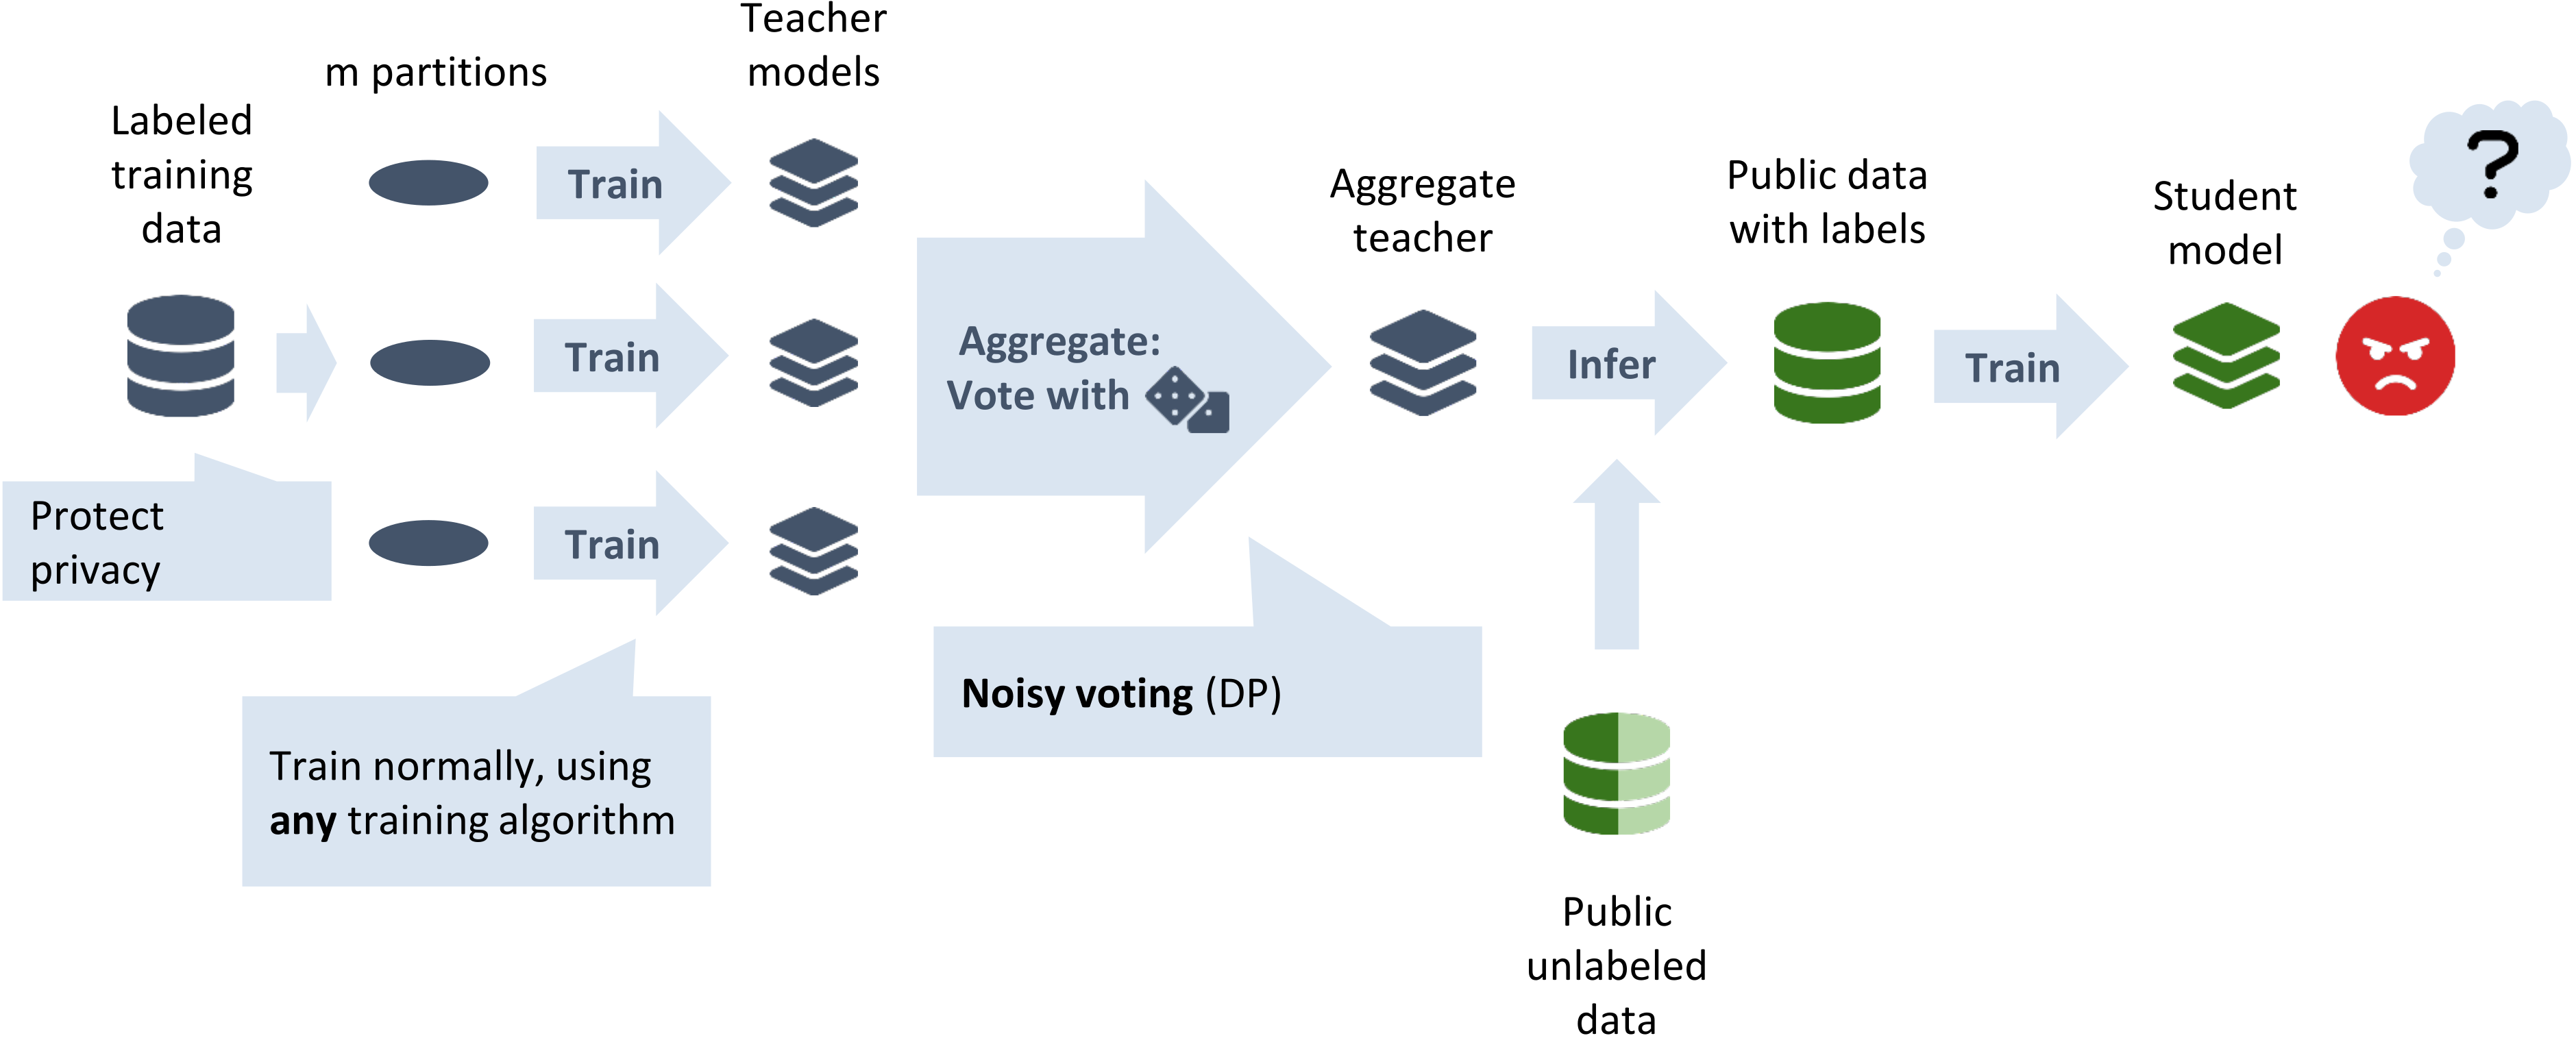
\includegraphics[width=\columnwidth]{img/pate.png}
Noisy voting: Add $\text{Laplace}(0,\frac{2}{\varepsilon})$-noise to each class count $n_c(x)$ before $\argmax$ ($n_c$ has $L_1$-sensitivity 2). Results in $N\varepsilon$-DP, where $N$ is the number of classifications we compute on the public unlabeled data.

    \section{Synthetic Data}
\textbf{Goal}: Dataset with same statistical properties \& provable DP guarantees\\
\textbf{Marginal}: \#Elements per attribute subset split by attribute domains ($L_2$-sensitivity: 1)\\
\textbf{Exponential Mechanism}: $\P\left[\Mo(\Do)=r\right] \propto exp(\epsilon\cdot q(\Do,r))$, $q$: quality score\\
\textbf{ProgSyn}: 1. Sample random noise $z\sim\No(0,I_p)$. 2. pass $z$ through genrative model $\Theta(z)$. 3. Obtain synthetic dataset $g_{\Theta}(z)$. 4. Adapt params $\Theta$ $\rightarrow$ $g_{\Theta}(z)$ close to $X$. 5. Fine-tune params $\Theta$ $\rightarrow$ $g_{\Theta}(z)$ satisfy additional constrains

    \section{Logical Properties}
\subsection*{DL2}
Idea: Translate properties $\phi$ into loss function $T$ and optimize.
For example, $\phi$ could be: $\|z-x\|_{\infty}<\epsilon \Rightarrow \|NN(z)-NN(x)\|_{\infty}<\delta$.

% Useful rules:
% \begin{itemize}
%     \item $x\Rightarrow y$ is equivalent to $\neg x \lor y$.
%     \item $\neg (x \lor y)$ is equivalent to $\neg x \land \neg y$.
%     \item $\neg (x \land y)$ is equivalent to $\neg x \lor \neg y$.
% \end{itemize}

\vspace*{1mm}
\renewcommand{\arraystretch}{1.1}
\begin{tabular}{ll}
    \hline
    $\phi $           & $T(\phi)$                            \\
    \hline
    $t_1 \leq t_2$    & $\max(0, t_1 - t_2)$                 \\
    $t_1 \neq t_2$    & $\mathbbm{1}_{\{t_1 = t_2\}}$        \\
    $t_1 = t_2$       & $T(t_1 \leq t_2 \land t_2 \leq t_1)$ \\
    $t_1 < t_2$       & $T(t_1 \leq t_2 \land t_1 \neq t_2)$ \\
    $\phi \lor \psi$  & $T(\phi) T(\psi)$                    \\
    $\phi \land \psi$ & $T(\phi) + T(\psi)$                  \\
    \hline
\end{tabular}
\vspace*{1mm}
$\forall x: T(\phi)(x) = 0 \Leftrightarrow x\ \text{satisfies}\ \phi$.

\subsection*{Training for Logical Properties}
Idea: Get the worst violation of $\phi$ and find $\theta$ that minimizes its effect. I.e. solve {$\min_\theta\mathbb{E}_{s \sim D} \big[ T(\phi)(z^*, s, \theta) \big]$} where {$z^* \in \argmin_z T(\lnot \phi)(z, s, \theta)$}.

In practice, restrict $z$ to a convex set with efficient projections (closed form). One can then remove the constraint from $\phi$ that restricts $z$ on the convex set and do PGD while projecting $z$ onto the convex set.

    \section{Individual Fairness}
\textbf{DEF:} A model $M$ is individually fair if for any similar $x,x'$ it produces similar outputs $M(x),M(x')$, e.g.
\begin{itemize}
    \item Lipschitz continuity: $\mu(M(x),M(x'))\le L\phi(x,x')$.
    \item Binary similarity: $\phi(x,x')\rightarrow M(x)=M(x')$.
\end{itemize}
% Then use DL2 to translate the similarity constraint into loss functions.

\subsection*{Fair Representation Learning:}
\begin{itemize}
    \item Data Regulator: Determines fairness criteria and data source(s), audits results.
    \item Data Producer: Computes the fair representation given data regulator criteria.
    \item Data Consumer: Trains the ML model given the sanitized data.
          Split models into an encoder $f_\theta$ (data producer) and a predictor $h_\psi$ (data consumer).
\end{itemize}

\subsection*{LCIFR}
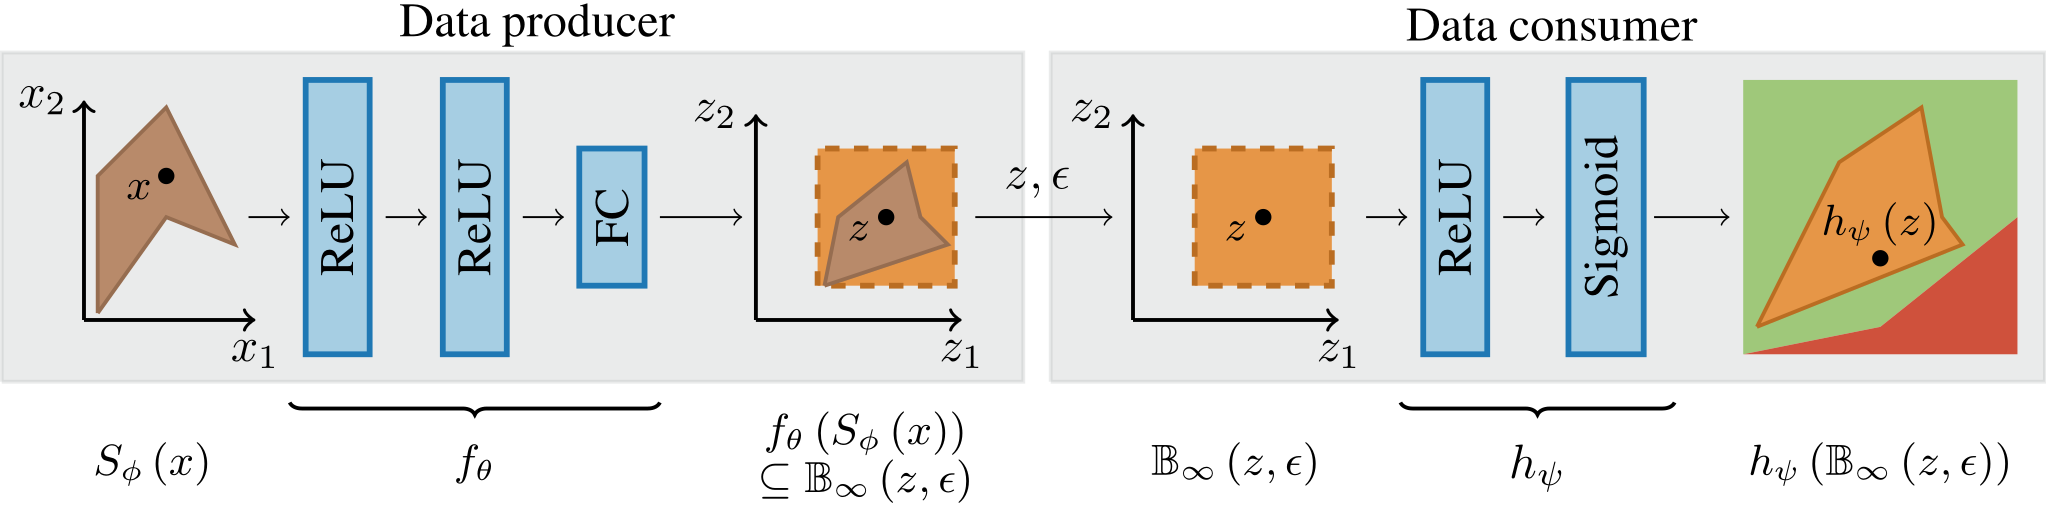
\includegraphics[width=1\columnwidth]{img/lcifr.png}
Consider binary $\phi,\mu$. 1. Encoder $f_\theta$ is trained s.t. $\phi(x, x') \Rightarrow \|f(x) - f(x')\|_\infty \leq \delta$ (with a combined loss ensuring informativeness of the representations) using DL2 (or $\delta$ is computed when encoded as MILP). 2. Use $L_\infty$-robustness training on encoded data for perturbations of magnitude $\delta$ and certify robustness. Gives certified individual fairness. Problem: Relies on NN verifiers so not scalable to real-world models.

\subsection*{LASSI}
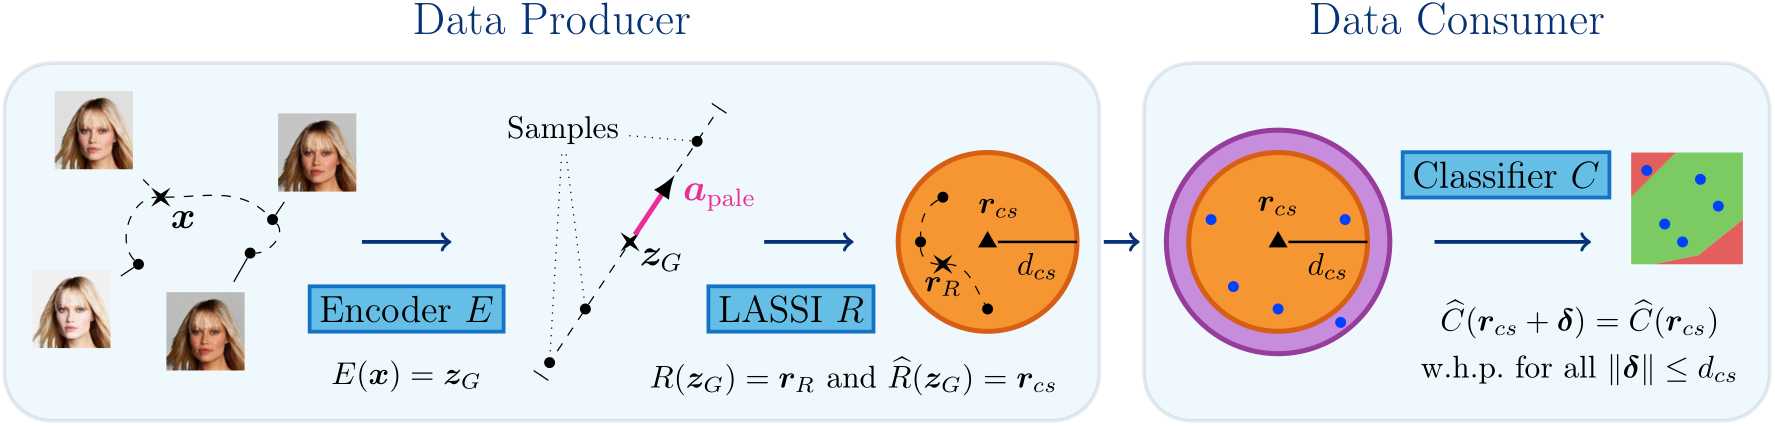
\includegraphics[width=1\columnwidth]{img/lassi.png}
1. Data producer uses center smoothing to get an encoder that provably maps all similar points close together with high probability. 2. Data consumer uses randomized smoothing to certify that all points within a certain radius get classified the same with high probability. Problem: Depends on quality of generative model.

\section{Group Fairness}
\textbf{Demographic Parity}\\
$P(\hat Y\mid G=0)=P(\hat Y\mid G=1)$\\
\textbf{Equalized Odds}\\
$P(\hat Y\mid G=0,Y=0)=P(\hat Y\mid G=1,Y=0)$\\
$P(\hat Y\mid G=0,Y=1)=P(\hat Y\mid G=1,Y=1)$\\
\textbf{Equal Opportunity}\\
$P(\hat Y\mid G=0,Y=1)=P(\hat Y\mid G=1,Y=1)$

\textbf{Approaches:}
\begin{itemize}
    \item Pre-processing: Debias the data, such that standard training yields a fair model. E.g. fair representation learning.
    \item In-training: Change the training pipeline to learn a fair model (on biased data). E.g. add soft fairness constraint to the loss.
    \item Post-processing: Modify predictions at inference time. E.g. different thresholds for different groups.
\end{itemize}

\subsection*{LAFTR}
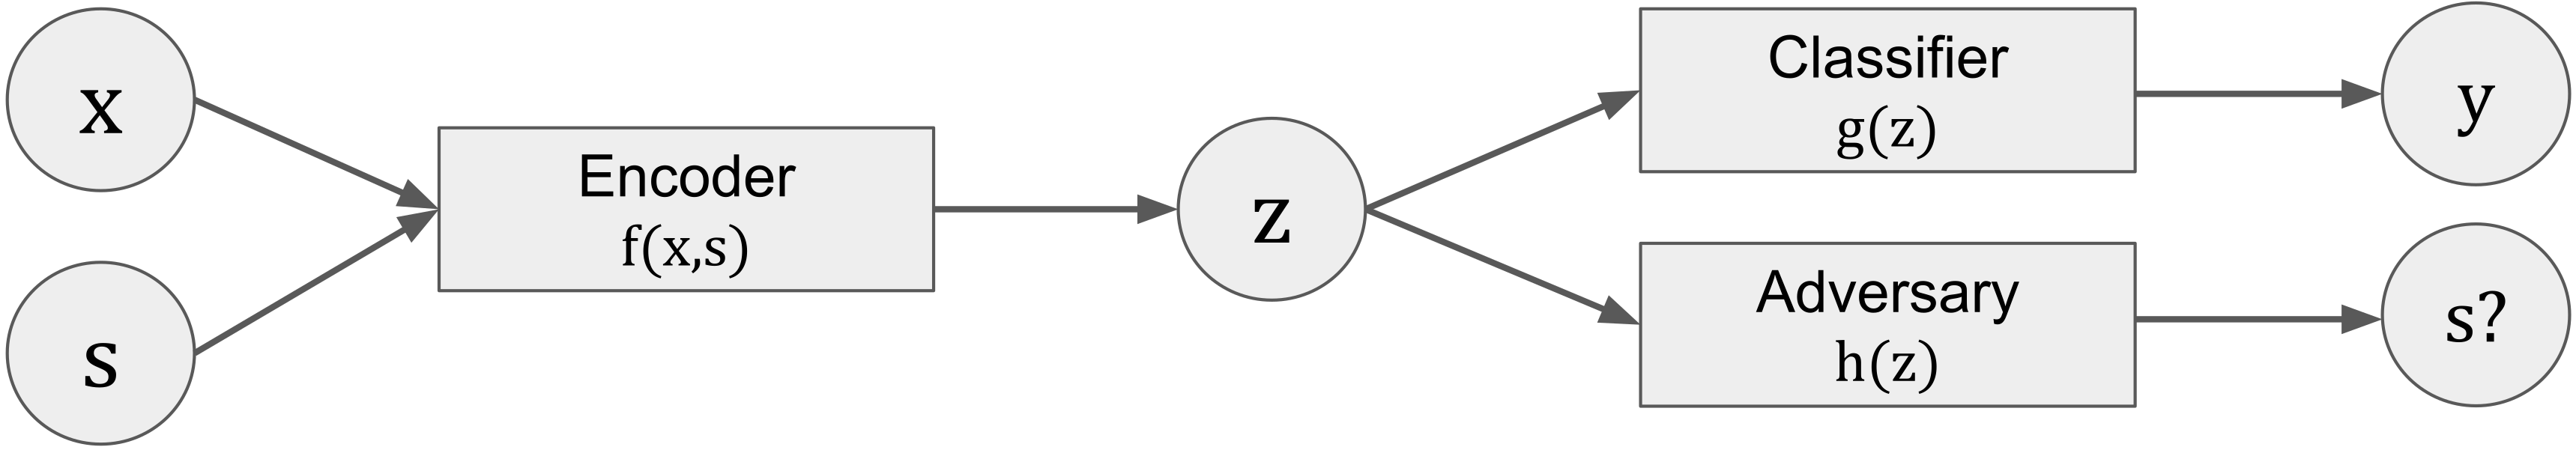
\includegraphics[width=1\columnwidth]{img/laftr.png}
Jointly trains an encoder $f$, classifier $g$, and adversarial classifiers $h$ by solving\\
$\min_{f,g}\max_{h\in\mathcal{H}} \mathcal{L}_{\text{clf}}(f,g)-\lambda \mathcal{L}_{\text{adv}}(f,h)$.\\
\textbf{Balanced Accuracy}\\
$\operatorname{BA}(h)=\frac{1}{2}\E_{Z_0}\left[1-h(z)\right]+\frac{1}{2}\E_{Z_1}h(z)$\\
$h^*=\argmax_h\operatorname{BA}_{Z_0,Z_1}(h)=\mathbbm{1}_{\{p_1(z)\geq p_o(z)\}}$\\
% % \vfill\null
% \columnbreak
\textbf{DP-Distance} (Relaxation of DP)\\
$\Delta^{\text{DP}}_{Z_0,Z_1}(g)=\left|\E_{Z_0}g(z)-\E_{Z_1}g(z)\right|$\\
$\Delta^{\text{DP}}_{Z_0,Z_1}(g)\leq2\operatorname{BA}_{Z_0,Z_1}(h^*)-1$\\
LAFTR estimates $\Delta^{\text{DP}}_{Z_0,Z_1}(g)$ given an adversary $h$. Fairness is overestimated (there may be better adversaries).

\subsection*{Fair Normalizing Flows}
Normalizing flows for a distribution $p(z)$ parameterize $z=f(x)$ where $x$ is sampled from a simple distribution $q(x)$ through an invertible transformation: $p(z)=q(f^{-1}(z))\left|\det{\partial_z f^{-1}}(z)\right|.$\\
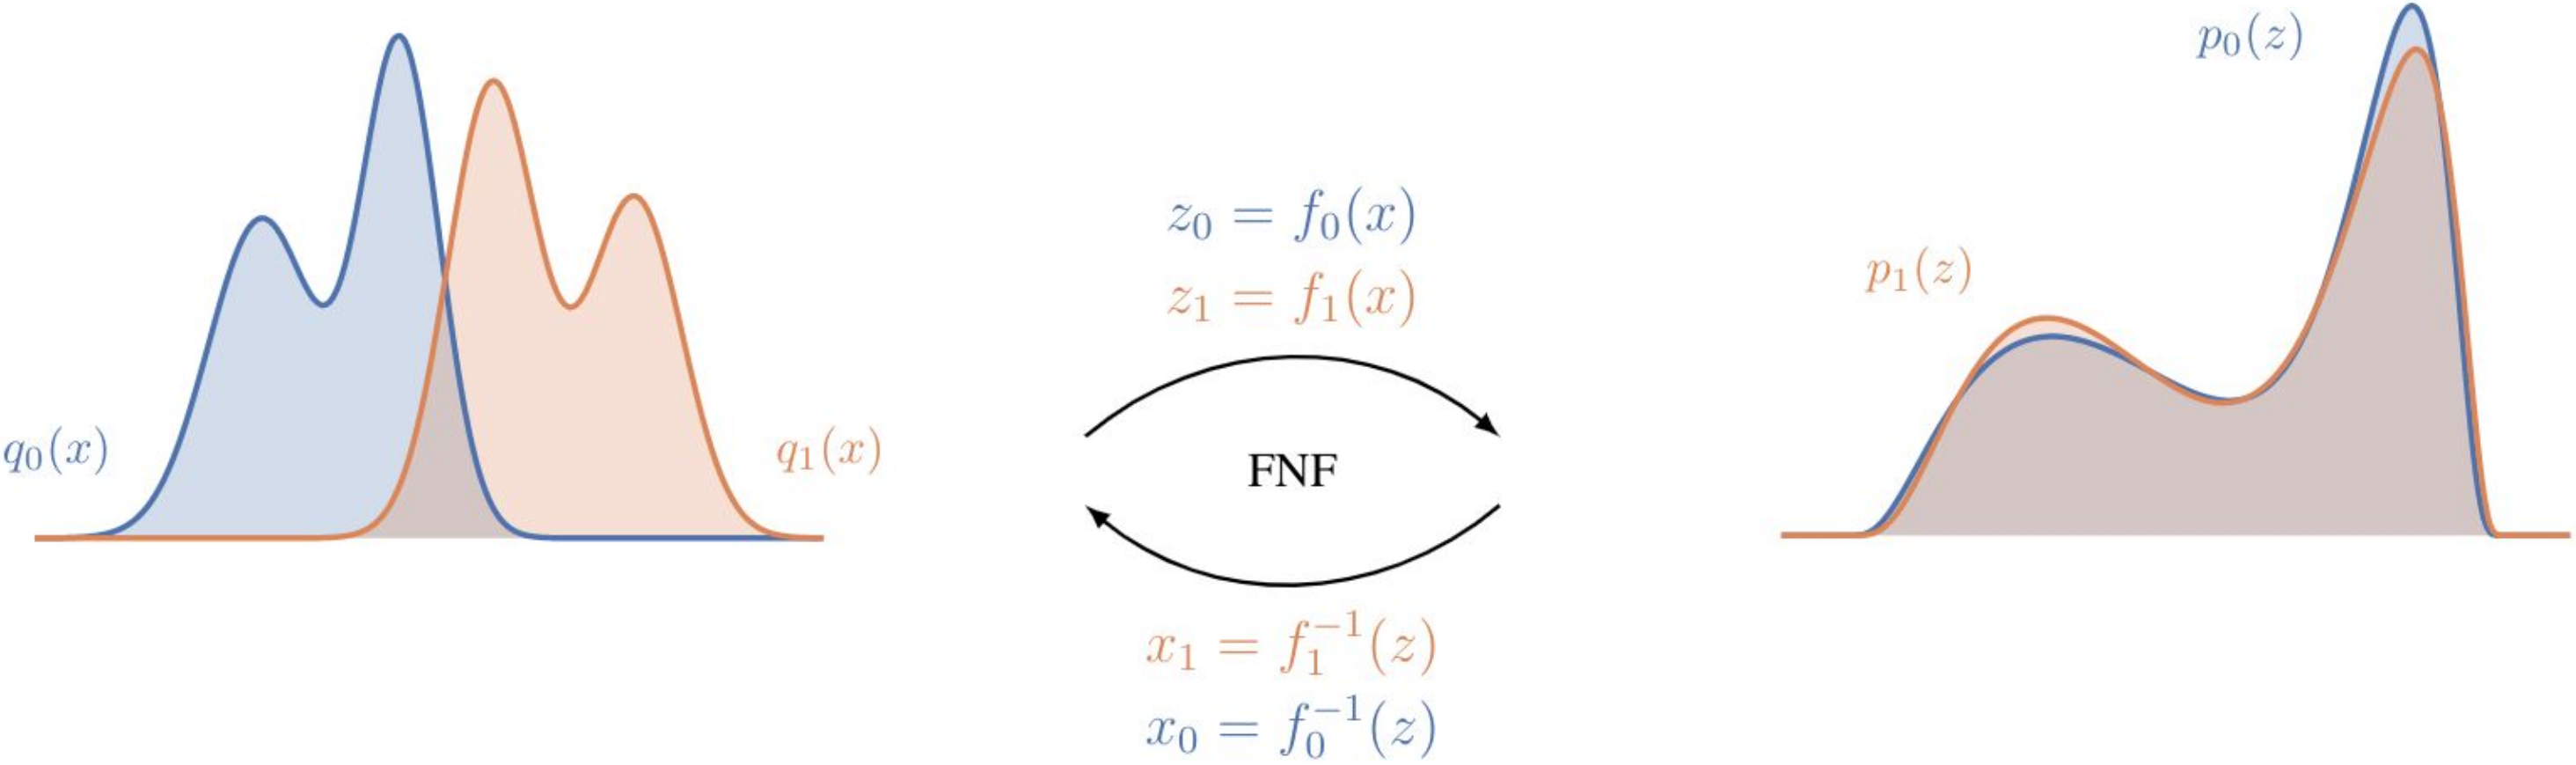
\includegraphics[width=1\columnwidth]{img/fnf.png}
FNF learns two flows $f_0,f_1$ as encoders for $Z_0,Z_1$. 1. Estimate densities $q_0, q_1$ for both groups. 2. Apply the encoder to get $z=f_0(x)$ (or $f_1(x)$), and use the flows and $q_0,q_1$ to get $p_0(z)$ and $p_1(z)$. 3. Use $p_0(z)$ and $p_1(z)$ to estimate the optimal adversary $h*$ and then upper bound its balanced accuracy with probability $1-\varepsilon$ (Hoeffding) 4. Use the inequality from LAFTR above to upper bound the DP-distance of any downstream classifier trained on representations z with probability $1-\varepsilon$.

To get tight bounds: train the flows to promote low accuracy of $h^*$ by minimizing $D_{KL}(p_0||p_1)+D_{KL}(p_1||p_0)$. \Warning The guarantees hold for the estimated $q_0,q_1$.

\subsection*{FARE}
Restrict representations $z$ to a finite set. This allows bounding $\operatorname{BA}_{Z_0,Z_1}(h^*)$ whp. directly. Use fairness-aware decision tree as encoder which is obtained by training a tree to have unbalanced leaves wrt. $y$ and uniform leaves wrt. $s$. Gives provable unfairness upper bound with no restrictive assumptions
    % \section{Miscellaneous}
\begin{itemize}
  \item Laplace: $f(x)=\frac{1}{2\sigma}e^{-\frac{|x-\mu|}{\sigma}}$
  \item Normal: $f(x)=\frac{1}{\sqrt{2\pi\sigma^2}}e^{-\frac{(x-\mu)^2}{2\sigma^2}}$
  \item $x\Rightarrow y$ is equivalent to $\neg x \lor y$
  \item DP: noise $\oplus$ $\rightarrow$ privacy $\oplus$ \& utility $\ominus$
  \item Carlini-Wagner: $\|.\|_{\infty}\rightarrow\sum_i \max(\eta_i-\tau,0)$
  \item Adversarial Accuracy: $\frac{\#\text{correct} - \#\text {adv\_examples}}{\#\text{samples}}$
  \item Cross entropy loss: $-\sum_i\sum_c y_{i,c}\log(p_{i,c})$
\end{itemize}

\end{multicols*}
\end{document}
